\documentclass{article}
\usepackage[utf8]{inputenc}
\usepackage{graphicx, amsmath, amssymb}
\usepackage{hyperref}
\graphicspath{ {./images/} }
\usepackage[dvipsnames]{xcolor}
\usepackage{titlesec}
\usepackage{tikz}
\usetikzlibrary{arrows.meta, positioning}
\DeclareMathOperator*{\KL}{KL}
\title{Generative Adversarial Networks}
\author{Sumit Singh}
\date{\today}

\begin{document}

\maketitle




%******************************************************
\section{Introduction}
%******************************************************





%******************************************************
\section{Variational Inference}
%******************************************************
 Variational Inference is a powerful technique in Bayesian Statistics and Machine Learning for approximating complex posterior distributions. \\
\textit{What are latent variables in Variational Inference?} \\
Latent variables are hidden/unobserved variables. Let us assume that $x = x_{1:n}$ are observations and $z = z_{1:m}$ are hidden variables. 
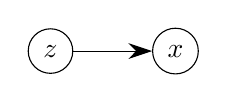
\begin{tikzpicture}[
  node/.style = {circle, draw, minimum size=0.5cm},
  >={Stealth[length=3mm, width=2mm]}  % arrow style
]
  % Define nodes
  \node[node] (z) {$z$};
  \node[node] (x) [right=1cm of z] {$x$};

  % Draw directed edge from z to x
  \draw[->] (z) -- (x);

\end{tikzpicture}
In probabilistic models, latent (hidden/unobserved) variables are 
variables that we do not directly observe (often denoted as $z$), but we assume they influence the observed data $x$. You do not observe $z$. You observe $x$. $x$ is governed by the hidden variable $z$. Hidden/Latent variables represent the underlying structure or ``explanatory factors" of the data. Given the observation, what is the code that generated this observation? That is the case with regression, classification, Topic Modeling.  Factor Analysis, Hidden Markov Models (HMM), Latent Dirichlet Allocation (LDA), and Structural Equation Modeling (SEM) are models that use latent variables. \\ 
\textbf{Generative Model Perspective}: The generative model is typically something like:
\begin{align*}
    p_\theta (x,z) = p_\theta(x|z) \cdot p_\theta (z)
\end{align*}
Here, $p_\theta (z)$ is the prior over the latent variable, and $p_\theta (x|z)$ is how we generate data given $z$. \\


The \textbf{marginal likelihood} of the data (what we really care about) is:
\begin{align*}
    p_\theta(x) = \int p_\theta (x,z) dz = \int_z p_\theta (x|z) p_\theta (z) dz 
\end{align*}
Usually, this integral is intractable for complex models. If $z$ is high dimensional, $p_\theta(x) = \int_z p_\theta (x|z) p_\theta (z) dz$ is intractable. That is one of the main obstacle in Graphical Models.
\begin{align*}
    \int \int \int \int \int \int \cdot \cdot \cdot \cdot \cdot dz
\end{align*}


\textbf{Posterior over Latent Variables ($p_\theta (z|x)$)} : What we really want in Bayesian inference is the posterior $p_\theta(z|x)$  -- how latent variables $z$ are distributed given the observed data $x$. But it is often intractable because it involves the marginal likelihood ($p_\theta (x)$) in the denominator.  
\begin{align*}
    p_\theta (z|x) = \frac{p_\theta (x|z) \cdot p_\theta (z)}{p_\theta (x)}
\end{align*}
$p(x|z)$ is easy to compute. $p_\theta (z)$ is the prior. $p_\theta (x)$, the marginal likelihood is hard to compute.
\\
In Bayesian Statistics, we often want to compute the posterior. Huge literature of graphical model or Bayesian Statistics is about approximating this marginal likelihood $p_\theta (x)$, an intractable quantity. There are many different techniques.
\begin{itemize}
    \item One line of technique is sampling-based methods, such as Monte Carlo Methods. Importance Sampling, MCMC Pseudo-Marginal / Particle MCMC, and Nested Sampling are different Monte Carlo Methods. Both Gibbs sampling and Metropolis Hastings are part of the MCMC category of approximate Bayesian inference. Gibbs sampling is a special case of Metropolis-Hastings. 
    \item Another set of techniques is Variational Inference
\end{itemize}
So instead, we approximate the true posterior with a more tractable distribution $q_\phi (z|x)$. This is where variational inference comes in. Variational Inference, in principle, means allowing us to transform this intractable quantity, $p(z|x)$, into an optimization problem. It is done by assuming that another distribution exists, which is tractable. Find the parameter of that one such that it is quite close to $p(z|x)$. If it is close to $p(z|x)$, I use it as a surrogate.\\
Assume that there is a $q(z)$. $q$ comes from a well behaved family (e.g., Gaussian). It is parameterized by $\phi$: $q_\phi (z|x)$. \\
We want to minimize the KL Divergence of this $q$ with my posterior:
\begin{align*}
    min \quad \KL_{\phi} (q_\phi (z|x) || p_\theta(z|x))
\end{align*}
If I can minimize this Kullback-Leibler Divergence  and find appropriate $\phi$s, the $q_\phi (z)$ is close to my posterior $p(z|x)$  and $q_\phi(z)$ is well behaved (it is from Gaussian). Hence, we will use $q_\phi(z)$ instead of $p_\theta (z|x)$. $\phi$ depends on $x$, it is a function of $x$. \\
It is not easy to minimize the Kullback-Leibler divergence:
\begin{align*}
    min \quad \KL_\phi (q_\phi (z|x) || p_\theta(z|x) )
\end{align*}
This is so because this Kullback-Leibler divergence depends on a quantity which is unknown : $p_\theta (z|x)$. The problem that we started with was: we do not know what's $p_\theta (z|x)$? Variational Inference is a way to get around this.\\ 
\subsection{KL Divergence}
Kullback-Leibler divergence measures similarity between two distributions. It comes from Information Theory. If $x$ is an event, the Information $I$ of and event $x$ is given by:
\begin{align*}
    I = - log(p(x))
\end{align*}
Higher Probability $\implies$ Lower Information. The information: ``the sun is going to rise in the east tomorrow" is a sure (very high probability) event with absolutely no information. While the information: ``There is going to be a meteor shower on a certian night" is a low probability event with high information. \\
\begin{align*}
    Entropy: \quad H = \mathbb{E}[I] = - \sum p(x) \cdot log(p(x))
\end{align*}
\begin{align*}
    D_{KL} (P||Q) = \sum_x P(x) \cdot log \frac{P(x)}{Q(x)} = \int_{- \infty}^{\infty} p(x) \cdot ln \frac{p(x)}{q(x)}
\end{align*}
\begin{align*}
    D_{KL}(Q||P) = \sum_x Q(x) \cdot log \frac{Q(x)}{P(x)} = \int_{- \infty}^{\infty} q(x) \cdot ln \frac{q(x)}{p(x)}
\end{align*}
\begin{align*}
    D_{KL} (P||Q) \neq D_{KL} (Q||P)
\end{align*}
\subsubsection{Kullback-Leibler Divergence of Bernouli}
Let $X \sim Bern(p_\alpha)$ and  $Y \sim Bern(p_\beta)$. What is the KL Divergence between them?
\begin{align*}
    KL(X,Y) &= \sum_x []
\end{align*}

\textit{How does Variational Inference work with Latent Variables?} \\
\begin{itemize}
    \item \textbf{Approximate Posterior (Variational Distribution)}
    \begin{itemize}
        \item We pick a parametric family for $q_\phi (z|x)$ (e.g., a Gaussian) that's easier to work with
        \item The goal is to make $q_\phi (z|x)$ as close as possible to the true posterior $p_\theta (z|x)$. The closeness is measured using KL divergence.
    \end{itemize}
    \item \textbf{Evidence Lower Bound (ELBO)}
    \begin{itemize}
        \item Instead of maximizing the intractable log-likelihood $log$ $p_\theta (x)$ directly, we maximize a lower bound called the ELBO
        \item The ELBO is:
        \begin{align*}
            \mathbb{E}_{q_\phi (z|x)} [log p_\theta (x|z)] - KL(q_\phi (z|x) || p_\theta (z))
        \end{align*}
    \end{itemize}
    \item \textbf{Reparameterization Trick}
\end{itemize}

%******************************************************
\section{Questions}
%******************************************************






%******************************************************
\section{Terms}
%******************************************************
Latent Model $\triangle$ Posterior Collapse $\clubsuit$ Variational Inference $\spadesuit$ Reparameterization Trick $\heartsuit$ Approximate Posterior (Variational Distribution) $\square$ Kullback-Leibler (KL) Divergence $\triangle$ Evidence Lower Bound (ELBO) $\clubsuit$ Probabilistic Graphical Models $\spadesuit$  Bayesian Neural Networks  $\heartsuit$ Variational Autoencoders
\section{References}
\begin{itemize}
    \item %% https://adamlineberry.io/vae-series/variational-inference?utm_source=chatgpt.com
    \item %% https://www.cs.princeton.edu/courses/archive/fall11/cos597C/lectures/variational-inference-i.pdf
    \item %% https://www.cs.cmu.edu/~epxing/Class/10708-15/notes/10708_scribe_lecture13.pdf
\end{itemize}
\end{document}